\clearpage
\VerdierPhysicalPageAnchor{0084}%
\VerdierSemanticAnchor{ch1-3-1-2-phi-definition-continuation}
following morphism of $\operatorname{tr}_1(C)$:

\VerdierSemanticAnchor{ch1-3-1-2-phi-diagram}
\begin{equation*}
  \Phi(f)=(0,p(f),a(f))
  \qquad
  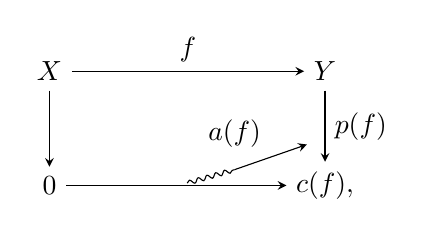
\begin{tikzpicture}[>=stealth,baseline=(current bounding box.center)]
    \node (X)  at (0,1.45) {$X$};
    \node (Y)  at (3.5,1.45) {$Y$};
    \node (Z)  at (0,0) {$0$};
    \node (Cf) at (3.5,0) {$c(f)\mathpunct{,}$};
    \draw[->] (X) -- node[above] {$f$} (Y);
    \draw[->] (X) -- (Z);
    \draw[->] (Y) -- node[right] {$p(f)$} (Cf);
    \draw[->] (Z) -- (Cf);
    \draw[decorate,decoration={snake,amplitude=0.8pt,segment length=3.3pt}]
      (1.75,0.03) -- (2.35,0.20);
    \draw[->] (2.35,0.20) -- node[above left] {$a(f)$} (3.27,0.52);
  \end{tikzpicture}
\end{equation*}

\VerdierSemanticAnchor{ch1-3-1-2-eq4}
\begin{equation}
  \begin{aligned}
    p(f)^i&=
      \begin{pmatrix}
        \operatorname{id}_{Y^i}\\[1mm]
        0
      \end{pmatrix}
      \colon Y^i\longrightarrow Y^i\oplus X^{i+1},\\[2mm]
    a(f)^i&=
      \begin{pmatrix}
        0\\[1mm]
        \operatorname{id}_{X^{i+1}}
      \end{pmatrix}
      \colon X^{i+1}\longrightarrow Y^i\oplus X^{i+1}.
  \end{aligned}
  \tag{3.1.2.4}
\end{equation}

\VerdierSemanticAnchor{ch1-3-1-2-phi-naturality}
An immediate calculation shows that $\Phi$ is a morphism from the identity
functor of the category $\operatorname{tr}_1(C)$ to the functor $sc$.

\VerdierSemanticAnchor{ch1-3-1-3}
\noindent\textbf{Proposition 3.1.3.}\quad
\emph{The morphism $\Phi$ makes the cone functor a left adjoint to the functor
$s$, i.e. for every object $X\xrightarrow{f}Y$ of
$\operatorname{tr}_1(C)$ and for every object $W$ of
$\operatorname{comp}(C)$, the canonical map defined by the morphism $\Phi$:}

\VerdierSemanticAnchor{ch1-3-1-3-hom-isomorphism}
\begin{equation*}
  \operatorname{Hom}_{\operatorname{comp}(C)}(c(f),W)
  \longrightarrow
  \operatorname{Hom}_{\operatorname{tr}_1(C)}
    \bigl((X\xrightarrow{f}Y),sW\bigr)
\end{equation*}
\emph{is an isomorphism.}

\VerdierSemanticAnchor{ch1-3-1-3-verification}
The verification is left to the reader.
\VerdierSemanticAnchor{ch1-3-1-3-s-fully-faithful}
Note that the functor $s$ is fully faithful and that consequently the functor
$cs$ is canonically isomorphic to the identity functor.
\VerdierSemanticAnchor{ch1-3-1-3-cs-identity}
In fact, with the chosen construction of the functor $c$, the functor $cs$ is
equal to the identity functor.
\VerdierSemanticAnchor{ch1-3-1-3-adjunction-reformulation}
The adjunction property of (3.1.3) can also be expressed as follows: the map
defined by the functor:

\VerdierSemanticAnchor{ch1-3-1-3-c-hom-isomorphism}
\begin{equation*}
  c\colon
  \operatorname{Hom}_{\operatorname{tr}_1(C)}
    \bigl((X\xrightarrow{f}Y),sW\bigr)
  \longrightarrow
  \operatorname{Hom}_{\operatorname{comp}(C)}(c(f),W)
\end{equation*}
is an isomorphism.

\VerdierSemanticAnchor{ch1-3-1-4}
\noindent\textbf{3.1.4.}\quad
We shall define a notion of homotopy in $\operatorname{tr}_1(C)$. Let:

\VerdierSemanticAnchor{ch1-3-1-4-homotopy-setup}
\begin{equation*}
  (g,h,a),(g',h',a')\colon
  (X\xrightarrow{f}Y)
  \rightrightarrows
  (X'\xrightarrow{f'}Y')
\end{equation*}
